\chapter{Formatting Text}

\section{Emphasis}

\section{Sizes}

The default text size is controlled by your document class.
It is usually ten points,\punckern\footnote{In most digital publishing,
one point is \otffrac{1}{72} of an inch.
In \LaTeX{}, for historical reasons, it is
\otffrac{100}{7227} of an inch.}
but this can be adjusted by passing additonal arguments to
\verb|\documentclass|.\punckern\footnote{The standard \LaTeX{} classes accept
\texttt{10pt}, \texttt{11pt}, or \texttt{12pt}.
KOMA Script classes accept arbitrary sizes with
\monobox{fontsize=<size>}.}
To scale text relative to this size, use the following commands:
\begin{leftfigure}
\lm
\renewcommand{\arraystretch}{1.5}
\begin{tabular}{l l}
\verb|\tiny| & \tiny Example Text \\
\verb|\scriptsize| & \scriptsize Example Text \\
\verb|\footnotesize| & \footnotesize Example Text \\
\verb|\small| & \small Example Text \\
\verb|\normalsize| & \normalsize Example Text \\
\verb|\large| & \large Example Text \\
\verb|\Large| & \Large Example Text \\
\verb|\LARGE| & \LARGE Example Text \\
\verb|\huge| & \huge Example Text \\
\verb|\Huge| & \Huge Example Text \\
\end{tabular}
\end{leftfigure}
There is some subtlety here that you may not have noticed.
\LaTeX's default type family, Latin Modern,\punckern\footnote{Latin Modern is
an OpenType rendition of \LaTeX's original type family, Computer Modern.}
comes in multiple \introduce{optical sizes}.
Smaller fonts have thicker strokes, exaggerated features,
and more generous spacing to improve legibility at their size.
\begin{leftfigure}
\fontspec{lmroman5-regular} If you magnify 5 point type
\fontspec{lmroman10-regular} and place the result next to normal 10 point type,
the differences are immediately noticeable.
\end{leftfigure}
Since this requires much more work from the type designer,
many digital typefaces---even professional ones---lack this
feature.\punckern\footnote{If you are fortunate enough \emph{to} have
a typeface with multiple optical sizes, \XeLaTeX{}
and \LuaLaTeX{} can make good use of them! See \chapref{fonts}.}

If you set {\small various} {\scriptsize sizes} {\sffamily\small or fonts}
on the {\footnotesize same line},
they will be aligned on the \introduce{baseline}:

\begin{adjustwidth}{2em}{2em}
\vspace{0.5\baselineskip minus 0.3\baselineskip}
\centering
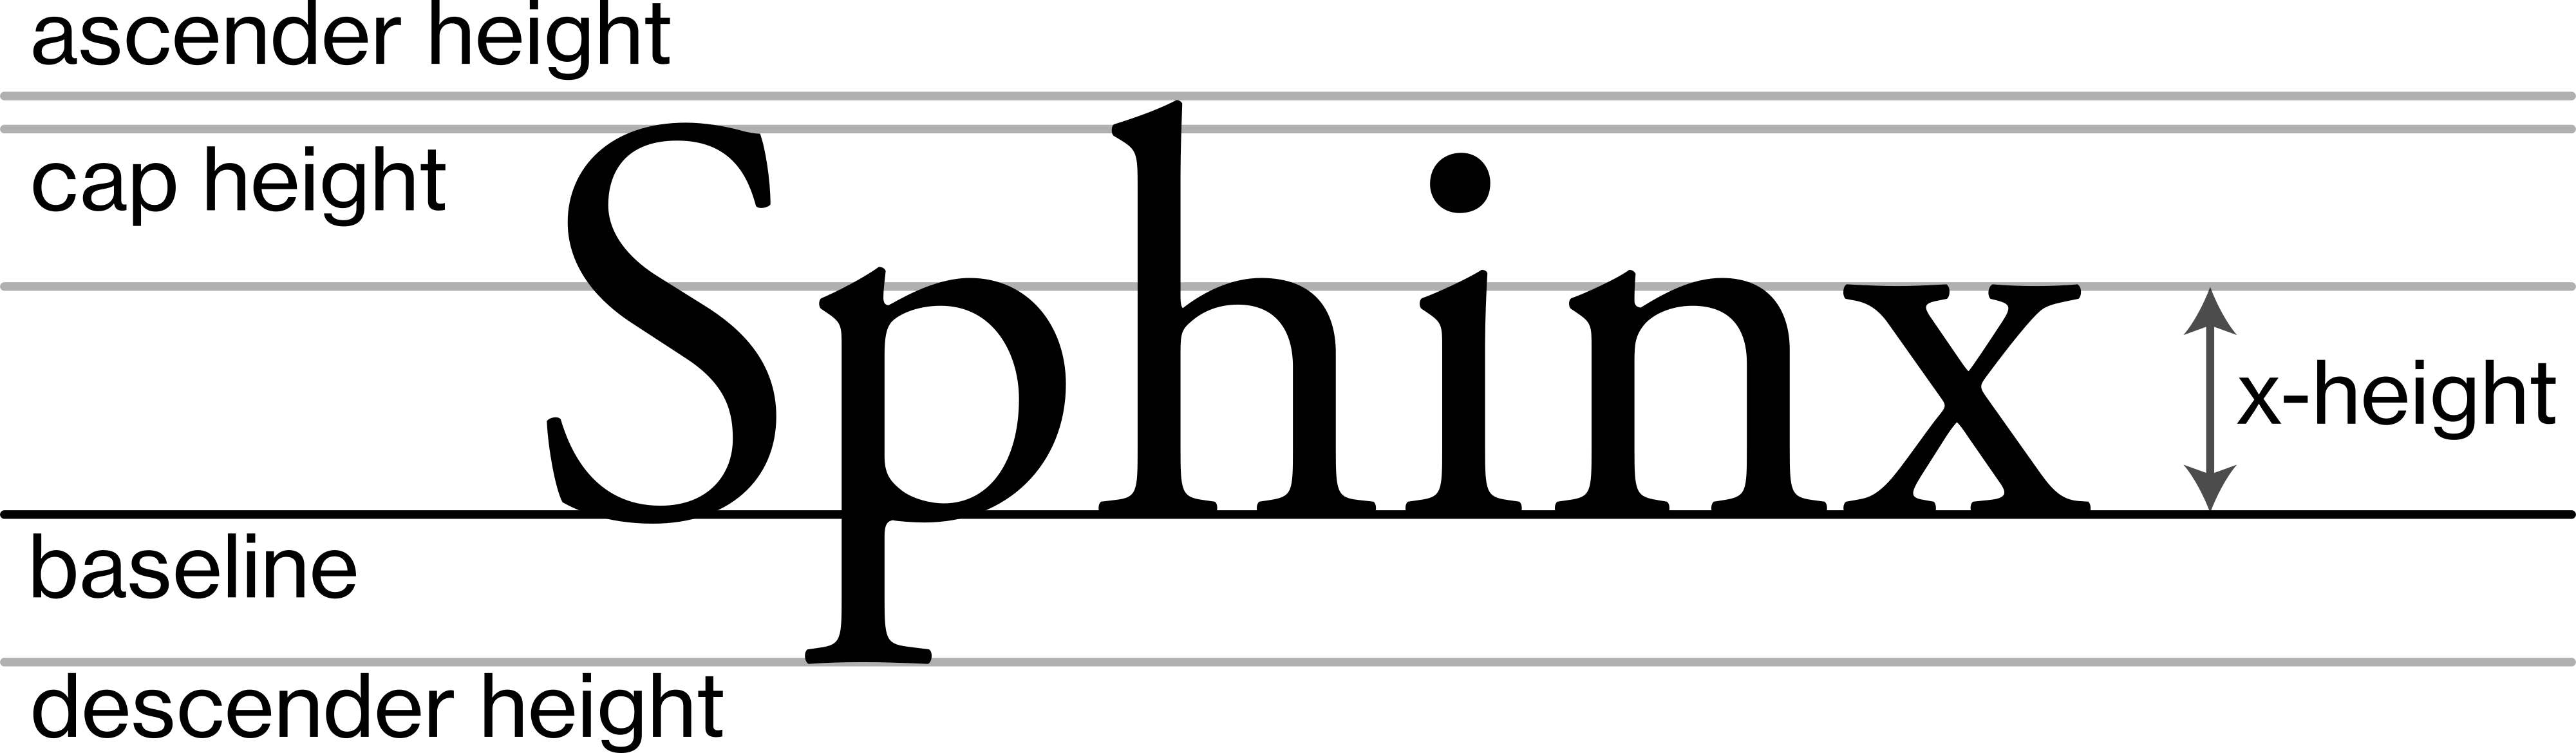
\includegraphics[keepaspectratio,width=0.65\textwidth]{heights.png}

\captionof{figure}{Common font metrics used in typography.
Text sits on the \introduce{baseline},
extends to the \introduce{ascender height},
and descends to the \introduce{descender height}.
The \introduce{cap height} refers to the size of uppercase letters,
and the \introduce{x-height} refers to the size of lowercase letters.
These values are different for each typeface,
and two set at the same point size might have very different heights.
Compare Helvetica to {\rmfamily Garamond}---the former has a much larger x-height.}

% For size reference:
%{\sffamily\fontsize{8pt}{8pt}\selectfont This is 8-point text.}
\vspace*{0.3\baselineskip minus 0.1\baselineskip}
\end{adjustwidth}

TODO: Talk about arbitrary sizes and leading.
